\secrel{azLinux}\secdown

Чтобы разобраться как можно собрать встраивамый \linux, в этом разделе описан
набор \make-файлов и файлов конфигурации для сборки минимального em\linux.
Это обрезанный форк проекта \href{https://github.com/user/cross}{Cross
Linux}, подробнее описанного в разделе \ref{cross}. Ограничено количество
поддерживаемого железа, упрощены конфигурационные файлы, минимизировано
количество библиотек и программных пакетов.

\bigskip

Изначально идея создания этой системы появилась из желания заменить тухлую
связку x86/DOS/Tur\-bo\-Pas\-cal на что-то

\begin{itemize}
  \item \emph{более переносимое}: на
 энергоэффективное ARM/MIPS-железо, в т.ч. (типа)отечественного производства,
\item \emph{стабильное}: с полноценной многозадачностью,
защитой памяти и данных, и
\item \emph{позволяющее использовать максимум возможностей аппаратуры}: большая
\ram, ECC, gcc-оп\-ти\-ми\-зи\-ро\-ван\-ный 32/64-битный код, USB, CAN, Ethernet,
WiFi, разнообразные носители данных, аппаратный watchdog.

\item Также большой интерес представляют \emph{десятки готовые библиотек} сжатия
и кодирования данных, численных методов, ЦОС, и обработки изображений, а также

\item множество \emph{готовых программ, доступных в исходных кодах}\note{для
использования как есть, изучения принципов работы и модификации под
собственные нужды}\ для выполнения различных полезных функций: сетевые серверы,
символьная математика, обработка данных,\ldots

\item Еще одна ключевая фича\ --- \emph{способность}\ \linux\ полностью
\emph{загружаться в \ram\ с \textbf{любых} носителей, в т.ч. заблокированных на
запись}. Это важно для случаев, когда возможны внезапные выключения питания:
вся система работает в \ram-диске, а корректность записи данных на изменяемые
носители можно гибко контролировать программно. При запуске после аварийного
выключения никаких проверок файловых систем не требуется, ОС стартует сразу, а
проверку/починку разделов данных возможно выполнять в фоновом режиме.

\item \emph{Время запуска системы}\ --- на x86 удалось экспериментально получить
время запуска \emph{0.2\,сек от загрузки ядра до начала выполнения
пользователького кода}.
Используя модульное ядро, возможно выполнить критический к времени запуска
пользовательский код до инициализации USB, сети, внешних носителей данных и
тяжелых сервисов.

\end{itemize}

\paragraph{Почему не BuildRoot}

Эта система сборки создавалась как \emph{максимально облегченный пакет
для решения узких задач}, и для освоения технологии кросс-компиляции.
Предполагается что функциональное наполнение не будет развиваться шире набора:

\begin{itemize}
  \item ядро (реального времени)
  \item $\mu$libc
  \item урезанная командная оболочка (busybox)
  \item несколько прикладных библиотек поддержки (сжатие, кодирование, базовая
  графика)
  \item пользовательский узкоспециализированный код на Си/\cpp
\end{itemize}

Расширять функционал, добавляя libQt, X Window, Apache, MySQL,\ldots, Gnome/KDE
и т.д. не планируется в принципе\ --- \emph{это система для решения узких
прикладных задач}\ на аппаратуре с минимальными ресурсами\note{особенно
интересны процессорные модули в DIMM форм-факторе, только CPU, RAM,
NAND и GPIO гребенка}. \emph{Интерактивная работа}\ с пользователем также
\emph{не предполагается}, доступна только командная консоль\note{ее можно
считать сервисным режимом}, и очень ограниченные графические и мультимедийные
возможности. Если ваши хотелки выходят за этот функционал, рекомендую сразу
уходить на использование ширко известной системы кросс-сборки \linux-систем под
названием \file{BuildRoot}\ref{buildroot}.

\secrel{Требования к системе сборки (\file{BUILD}-хост)}

Требования жесткие\ --- 2х-ядерный процессор, 2+\,Гб \ram, для 4+\, Гб \ram\
нужен 64х-битный дистрибутив \linux\ (рекомедую Debian), и естественно никаких
виртуалок.
Возможна установка системы на флешку, в этом случае требования к \ram\ еще более
ужесточаются\ --- потребуется каталоги с временными файлами смонтировать как
\file{tmpfs}:

\lst{добавить в \file{/etc/fstab}}{}{azlin/doc/fstab.txt}

Можно попытаться сделать \term{билд-сервер}\ и на худшем железе, но будьте
готовы к тормозам или внезапному окончанию памяти\ --- ресурсоемка сборка
тяжелых библиотек типа \pack{libQt}\ или крупных пакетов типа \pack{gcc}.

Вы можете попробовать поставить \linux\ на виртуалку, на флешку, и на жесткий
диск (если найдете место) и оценить возможности этих вариантов на сборке пакета
\pack{gcc0}. При сборке с флешки на ноутбуке с 2\,Гб \ram\ мне для сборки
\pack{gcc0}\ пришлось временно размонтировать \file{cross/src}, сделать
\file{./mk.rc \&\& make gcc ramclean}, а потом примонтировать \file{tmpfs}\
опять на \file{src}.

Сборка под MinGW/Cygwin совершенно неживая. Если совсем никак без винды\ ---
используйте виртуалки, и будьте готовы ждать.

\secrel{Понятие \term{пакет}}

Прежде чем продолжить, введем понятие \termdef{пакет}{пакет}. В az\linux\
\term{пакетом}\ называется одна или несколько частей скриптов сборки,
обозначаемых именем. В чем-то это похоже на бинарные пакеты обычных
дистрибутивов \linux\ --- чтобы добавить в систему какой-то функционал, мы
устанавливаем \term{бинарный пакет}.
Но есть и отличие: пакет дистрибутива это реальный архивный файл, содержащий в
себе файлы программ, данных; в az\linux\ пакет\ --- виртуальная штука с именем.

Просматривая файлы в каталоге \file{mk/}, легко найти имена пакетов по шаблону:

\begin{verbatim}
.PHONY: somename
somename: [зависимые файлы]
    [команда1]
    ...
\end{verbatim}

Если вы запустите команду:

\begin{verbatim}
cd ~/az ; ./mk.rc && make somename
\end{verbatim}

запустится \termdef{сборка пакета}{сборка пакета}\ \pack{somename}.

Но не нужно забывать, что кроме этой секции в \file{.mk}, существуют зависимости
между файлами, при работе команд сборки динамически создаются и изменяются
файлы, иногда что-то скачивается из \internet а\ --- все эти процессы тоже
входят в пакет.

\bigskip
Часть пакетов не связана со сборкой программ, а выполняют служебные функции,
поэтому для них правильнее будет фраза \term{запуск пакета}.

\bigskip
Все действия выполняются с помощью команды \pack{make}. Обратите особое
внимание на то, что \file{Makefile}\ собирается скриптом \pack{mk.rc}\ из частей
в каталоге \file{mk/}, поэтому \emph{если вы что-то меняете в скриптах, не
забудьте сначала запустить \pack{./mk.rc}}.

\lstx{mk.rc}{}{../azlin/mk.rc}{rc}\index{azLinux!скрипт!mk.rc}

\secrel{Клонирование проекта \pack{az\linux}} \label{azclone}

При необходимости вносить правки\note{что естественно\ --- вам потребуется
добавлять свои пакеты и поддержку железа}\ работайте с вашим
собственным форком на GitHub.

Получите клон пакета из репозитория:

\begin{verbatim}
cd ~ ; git clone --depth=1 -o gh https://github.com/user/azlin az
\end{verbatim}

При необходимости обновитесь:

\begin{verbatim}
cd ~/az ; git pull
\end{verbatim}

\secrel{Общий порядок сборки}

Каждый пакет собирается командой:

\begin{verbatim}
./mk.rc && make [HW=rpi] [APP=clock] <package>
\end{verbatim}

\begin{enumerate}
  \item \pack{dirs} создание дерева каталогов \ref{azdirs}
  \item \pack{gz} закачка архивов исходников \ref{azgz}
  \item \pack{tc} сборка кросс-компилятора \ref{aztc}
  \begin{enumerate}
    \item \pack{binutils} ассемблер, линкер и утилиты \ref{azbinutils}
    \item \pack{cclibs} библиотеки для сборки \pack{gcc} \ref{azcclibs}
    \item \pack{gcc0} сборка минимального кросс-компилятора Си \ref{azgcc0}
  \end{enumerate}
  \item \pack{core} сборка основной системы \ref{azcore}
  \begin{enumerate}
    \item \pack{kernel} ядро \linux\ \ref{azkernel}
    \item \pack{ulibc} библиотека \pack{uClibc} \ref{azulibc}
    \item \pack{busybox} набор утилит \pack{busybox} \ref{azbb}
    \item \pack{gcc} пересборка полного кросс-компилятора Си/\cpp \ref{azgcc}
  \end{enumerate}
  \item \pack{libs} сборка библиотек \file{\$\{LIBS\}} \ref{azlibs}
  \item \pack{apps} сборка прикладных пакетов \file{\$\{APPS\}} \ref{azapps}
  \item \pack{user} сборка пользовательского кода \ref{azuser}
  \item \pack{root} формирование корневой файловой системы \ref{azroot}
  \item \pack{boot} сборка загрузчика \ref{azboot}
   \pack{syslinux}/\pack{grub}/\pack{uboot}
  \item \pack{emu} запуск собранной системы в эмуляторе \ref{azemu}
  \item \pack{netboot} сетевая загрузка \ref{aznetboot}
  \item \pack{firmware} прошивка на устройство \ref{azfirmware}
\end{enumerate}

\secrel{Фиксация переменных}

Если вам требуется собрать систему со значениями переменных, отличающихся от
тех, которые прописаны в make-файлах, при запуске \emph{всех}\ пакетов нужно
указывать трюбуемые значения в командной строке. Это позволить легко выбрать
нужный вам вариант сборки.

\begin{verbatim}
./mk.rc && make HW=rpi APP=clock distclean dirs tc core libs apps boot root
\end{verbatim}

При таком указании все переназначения для этих переменных игнорируются, поэтому
возможны некоторые сложности с указанием например опций оптимизации.

\secrel{\pack{dirs}: Создание дерева каталогов} \label{azdirs}

После загрузки или обновления запустите пакет \pack{dirs}:

\begin{verbatim}
$ ./mk.rc && make dirs
mkdir -p /home/user/Azbuka/azlin/gz /home/user/Azbuka/azlin/src
/home/user/Azbuka/azlin/tmp /home/user/Azbuka/azlin/x86_64-linux-gnu
/home/user/Azbuka/azlin/qemu386-clock /home/user/Azbuka/azlin/qemu386-clock/boot
\end{verbatim}
\begin{verbatim}
$ ls -la
итого 72
-rwxr-xr-x 1 user user   121 Дек  8 11:43 mk.rc
drwxr-xr-x 2 user user  4096 Дек  8 11:43 mk
drwxr-xr-x 2 user user  4096 Дек  8 11:43 app
drwxr-xr-x 2 user user  4096 Дек  8 11:43 hw
drwxr-xr-x 2 user user  4096 Дек  8 11:43 cpu
drwxr-xr-x 2 user user  4096 Дек  8 11:43 arch
drwxr-xr-x 2 user user  4096 Дек  8 13:26 gz
drwxr-xr-x 2 user user  4096 Дек  8 11:43 app
drwxr-xr-x 3 user user  4096 Дек  8 13:26 qemu386micro
drwxr-xr-x 2 user user  4096 Дек  8 13:26 qemu386micro.cross
-rw-r--r-- 1 user user   147 Дек  8 11:43 README.md
-rw-r--r-- 1 user user 17699 Дек  8 13:25 azlin.tex
drwxr-xr-x 2 user user  4096 Дек  8 13:26 src
drwxr-xr-x 2 user user  4096 Дек  8 13:26 tmp
-rw-r--r-- 1 user user  2087 Дек  8 13:26 Makefile
\end{verbatim}

Пакет \pack{dirs}\ прописан в файле

\lstx{mk/dirs.mk}{}{../azlin/doc/dirs.mk}{mk}\index{azLinux!пакет!dirs}

Встроенная переменная \file{PWD}\ содержит полное имя каталога, из которого был
запущен \pack{make}.

\bigskip
Каталог зеркала архивов исхоных текстов программ

\lstx{GZ}{}{../azlin/doc/gz.dirs}{mk}\index{azLinux!переменная!GZ}

Каталог распаковки исходных текстов: некоторые пакеты должна собираться в дереве
исходников

\lstx{SRC}{}{../azlin/doc/src.dirs}{mk}\index{azLinux!переменная!SRC}

Каталог out-of-tree сборки: остальные пакеты умеют собираться вне дерева
исходников, если хватает \ram\ этот каталог удобно монировать как \file{tmpfs}

\lstx{TMP}{}{../azlin/doc/tmp.dirs}{mk}\index{azLinux!переменная!TMP}

Переменная \file{BUILD}\ задает \term{триплет}\ системы, на которой вы
собираете: x86\_64-linux-gnu, i686-linux-gnu или что-то подобное. Для получения
триплета используется подстановка строки, выдаваемой запуском \pack{gcc}.

\lstx{BUILD}{}{../azlin/doc/build.dirs}{mk}\index{azLinux!переменная!BUILD}

Каталог в который собирается кросс-компилятор. Используется триплет
рабочей \linux-системы.

\lstx{TC}{}{../azlin/doc/tc.dirs}{mk}\index{azLinux!переменная!TC}

Каталог целевой \file{rootfs}. Отдельно прописан загрузочный каталог, в который
будет записываться собранное ядро, образ \term{initrd}, бинарники и конфиги
загрузчика. Имя \file{ROOT}\ создается из двух переменных, описанных далее: имя
аппаратной платформы \file{HW}\ref{azhw}\ и имени приложения
\file{APP}\ref{azapp}.

\lstx{ROOT/BOOT}{}{../azlin/doc/root.dirs}{mk}
\index{azLinux!переменная!ROOT}\index{azLinux!переменная!BOOT}

Список всех рабочих каталогов в одной переменной:

\lstx{DIRS}{}{../azlin/doc/dirs.dirs}{mk}\index{azLinux!переменная!DIRS}

\secrel{\pack{gz}: Загрузка архивов исходников} \label{azgz}

\lstx{mk/gz.mk}{}{azlin/mk/gz.mk}{mk}

\secrel{APP: Приложение}\label{azapp}

\term{Приложение}\ --- короткое кодовое название вашего варианта сборки системы
в целом.

Приложение задается в файле \file{mk/head.mk}\ через
переменную \file{APP}, доступные значения:

\begin{enumerate}
  \item \pack{micro}: минимальная версия системы, только командная консоль
  \item \pack{clock}: простые \linux-powered электронные часы
\end{enumerate}

Значение переменной \file{APP}\ по умолчанию задано в \file{mk/head.mk}:

\lstx{APP @ hw/head.mk}{}{../azlin/doc/app.mk}{mk}
\index{azLinux!настройка!приложение}
\index{azLinux!переменная!APP}

Если вам нужно собрать другое приложение, вы можете переопределить значение из
командной строки при запуске \emph{всех}\ пакетов:

\begin{verbatim}
./mk.rc && make APP=micro distclean dirs tc core libs apps
\end{verbatim}

В \file{app/\$\{APP\}.mk}\ в переменных задаются:

\begin{itemize}
  \item \file{LIBS}: набор используемых библиотек
  \item \file{PACKS}: набор используемых программных пакетов \ref{azpacks}
\end{itemize}

\lstx{app/micro.mk}{}{../azlin/app/micro.mk}{mk}\index{azLinux!приложение!micro}

\lstx{app/clock.mk}{}{../azlin/app/clock.mk}{mk}\index{azLinux!приложение!clock}

\secrel{HW: Поддерживаемое железо}\label{azhw}\index{azLinux!железо}

Конфигурация целевого железа задается в файле \file{mk/head.mk}\ через
переменную \file{HW}, доступные значения приведены в таблице:

\noindent
\begin{tabular}{|l| l l|l l l l l l|l|}
\hline
HW & CPU & ARCH & RAM & HD & SD & USB & Eth & WiFi & GPIO \\
\hline
qemu386 & i486sx & i386 & 32M+ & \uncheckbox\ IDE & & \uncheckbox & ne2k &&\\
eeepc701 & CeleronM & i386 & 512M+ & \uncheckbox\ SSD & \uncheckbox\
SD & \checkbox & A?? & \uncheckbox\ AR2425 &\\
gac1037 & Celeron1037U & x86\_64 & 1G+ & \uncheckbox\ SATA & & \checkbox &
2$\times$RTL8111 &&\\
\hline
qemuARM & & arm & 32M+ &&&&&&\\
cubie1 & AllWinnerA10 & armhf & 1G && \uncheckbox\ $\mu$SD & \checkbox &&&\\
rpi & BCM2835 & armel & 512M && \uncheckbox\ SD&\checkbox&&&\\
\hline
qemuMIPS & &mips& 32M+ & & & & &&\\
mr3020 & AR7240 &mips& 32M & 4M & & \checkbox && \uncheckbox\ AR9331 &\\
vocore & RT5350 &mips& 32M & 8M & & \uncheckbox
&& \uncheckbox\ SoC &\\
bswift && AR9331 &mips& 64M & 16M & \uncheckbox\ & & & 20+ \\
\hline
\end{tabular}

\lstx{mk/head.mk}{}{../azlin/mk/head.mk}{mk}

\secrel{i386}\secdown\index{azLinux!железо!i386}

Персоналки с архитектурой \file{i386}\ --- самое сложное семейство с точки
зрения поддержки. Комбинации процессоров, материнских плат и плат расширений
дают сотни вариантов конфигураций, в т.ч. десятки моделей компьютеров в формате
PC/104 и промышленных панелей. Особенно доставляет тот факт, что 95\% периферии
имеет закрытые бинарные драйвера только для \win, поэтому будьте аккуратны с
выбором железа.

\secrel{qemu386: эмулятор QEMU}

\lstx{hw/qemu386.mk}{}{../azlin/hw/qemu386.mk}{mk}\index{azLinux!железо!QEMU}

\secrel{eeepc701: ASUS Eee PC 701}

\lstx{hw/eeepc701.mk}{}{../azlin/hw/eeepc701.mk}{mk}\index{azLinux!железо!ASUS Eee PC 701}

\secrel{gac1037: Gigabyte GA-C1037UN-EU rev.2}

\begin{tabular}{p{0.45\textheight} p{0.45\textheight}}
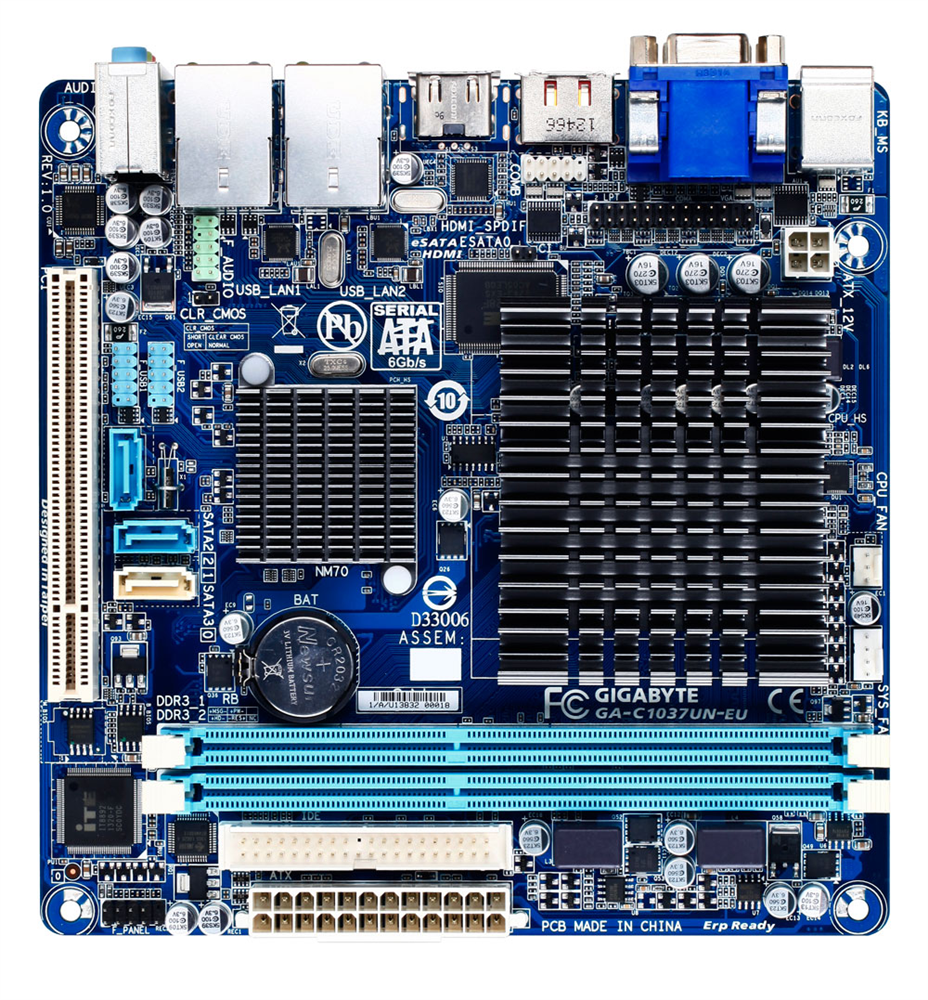
\includegraphics[height=0.45\textheight]{azlin/doc/gac1037.jpg} &
\begin{tabular}{l l}
CPU & Celeron 1037U \\
\ram & 2 $\times$ DDR3, max 16G, 2 канала \\
чипсет & Intel NM70 \\
сеть & 2 $\times$ Realtek® GbE 1Gb (rtl8111) \\
HDD & 2 $\times$ SATA2 (3Gb/s), 1 $\times$ SATA3 (6Gb/s), 1 $\times$ eSATA\\
USB & 6 $\times$ USB3.0 \\
видео & IntelGMA, выходы на VGA D-Sub и HDMI 1.4\\
аудио & Realtek ALC887 (HDA) \\
PCI & $\times$1 \\
&\\
\end{tabular}
\\
\end{tabular}

В качестве варианта 64-битной платформы взята портативная материнка для
неттопов: Gigabyte GA-C1037UN-EU. На ней возможны два варианта сборки:

\begin{enumerate}
  \item \emph{x86\_64/x64}: нативный \verb|CPU=Celeron1037u|
  \item \emph{i686/x32}: режим соместимости со старыми процессорами
  \verb|CPU=i686|
\end{enumerate}

\url{http://www.ixbt.com/news/hard/index.shtml?17/33/31}

\clearpage
На текущий момент эта материнка\ --- оптимальный вариант для офисного, рабочего
неигрового компьютера, или базы для изготовления мобильной рабочей станции в
миникейсе: комплект из GA-C1037UN-EU и блока питания стоит порядка 5 тыс.руб,
при этом возможна установка до 2$\times$8G \ram, что пока недоступно на дешевых
ноутбуках. \emph{Но\ --- \textsc{отвратительный} радиатор на мосте NM70, нагрев
до $70^{o}C$, в обязательном порядке делать сквозную продувку корпуса \textbf{до
включения материнки}.}

\begin{tabular}{l l}
материнская плата& GA-C1037UN-EU rev.2 \\
CPU& Celeron 1037U (впаян) \\
охлаждение& \emph{отвратительное, обязательны кулера на все чипы и сквозная
продувка корпуса},
\\
\ram& 1$\times$8G DDR3 (в планах 2$\times$8G) \\
HDD & \emph{нет}, используется флешка 8G USB3 Transcend JF750 (возможно SATA
SSD) \\
TFT & китайский 3.5'' автомониторчик + конвертер HDMI2RCA на случай\\&
посмотреть видеовывод, обычно везде где я использую эту поделку,\\& есть VGA
монитор или хотя бы большой телевизор\\
электропитание& БП Hipro HPE-350W + автоинвертор\\& батарея не требуется, под
боком всегда есть 220 или 12\,В\\
& по необходимости в транспорт грузится пара заряженных автоаккумуляторов\\
\end{tabular}
\bigskip

\lstx{hw/gac1037.mk}{}{../azlin/hw/gac1037.mk}{mk}\index{azLinux!железо!Gigabyte GA-C1037UN-EU}

\secup

\secrel{ARM}\secdown

\secrel{qemuARM: эмулятор QEMU}
\lstx{hw/qemuARM.mk}{}{../azlin/hw/qemuARM.mk}{mk}\index{azLinux!железо!QEMU}
\secrel{cubie1: Cubie Board v.1}
\secrel{rpi: Raspberry Pi model B}

\secup

\secrel{MIPS}\secdown
\secrel{qemuMIPS: эмулятор QEMU}
\lstx{hw/qemuMIPS.mk}{}{../azlin/hw/qemuMIPS.mk}{mk}\index{azLinux!железо!QEMU}
\secrel{mr3020: роутер MR3020}
\href{http://wiki.openwrt.org/ru/toh/tp-link/tl-mr3020}{mr3020}
\secrel{vocore: VoCore} \index{azLinux!железо!VoCore}
\href{http://vocore.io/}{vocore}
\secrel{bswift: BlackSwift} \index{azLinux!железо!BlackSwift}
\href{http://habrahabr.ru/post/242731/}{bswift}
\secup

\secrel{CPU: Конфигурации процессоров}\secdown

Настройки на процессор задаются в файле \file{cpu/\$\{CPU\}.mk}.

\begin{tabular}{p{0.15\textwidth} p{0.8\textwidth}}
\file{ARCH} & архитектура целевой системы, используется при конфигурировании
ядра \\
\file{TARGET} & \term{триплет целевой системы}, параметр задает тип целевой
системы при сборке кросс-компилятора и используется во всех скриптах
\pack{configure}\ при сборке остальных пакетов \\
\file{CFG\_CPU} & параметры при сборке кросс-компилятора \\
\file{CPU\_FLAGS} & параметры \pack{gcc}\ для оптимизации кода \\
\end{tabular}

\secrel{i386}

\lstx{cpu/i486sx.mk}{}{azlin/cpu/i486sx.mk}{mk}
\index{azLinux!железо!i486sx}

\lstx{cpu/CeleronM.mk}{}{azlin/cpu/CeleronM.mk}{mk}
\index{azLinux!железо!CeleronM}

\lstx{cpu/Celeron1037U.mk}{}{azlin/cpu/Celeron1037U.mk}{mk}
\index{azLinux!железо!Celeron1037U}

\secrel{ARM}
\secrel{MIPS}

\lstx{cpu/AR7240.mk}{}{../azlin/cpu/AR7240.mk}{mk}\index{azLinux!железо!AR7240}

\lstx{cpu/RT5350.mk}{}{../azlin/cpu/RT5350.mk}{mk}\index{azLinux!железо!RT5350}

\secup

\secrel{Пакеты}\secdown\label{azpacks}

\secrel{\file{versions.mk}: Версии пакетов}\label{azpackver}

\secrel{\pack{tc}: кросс-компилятор}

\lstx{mk/versions.mk}{}{azlin/doc/versions.cross}{mk}

\secrel{\pack{core}: ядро}

\lstx{mk/versions.mk}{}{azlin/doc/versions.core}{mk}

\secrel{\pack{boot}: загрузчики}

\lstx{mk/versions.mk}{}{azlin/doc/versions.boot}{mk}

\secrel{\pack{libs}: библиотеки}

\lstx{mk/versions.mk}{}{azlin/doc/versions.libs}{mk}

\secrel{\pack{tc}: сборка кросс-компилятора} \label{aztc}

\lstx{}{}{azlin/mk/cross.mk}{mk}

\secrel{\pack{binutils}: ассемблер, линкер и утилиты} \label{azbinutils}

\begin{tabular}{l l}
--target=\$(TARGET)& триплет целевой платформы\\
\$(CFG\_ARCH)&параметры архитектуры\\
\$(CFG\_CPU)&параметры процессора\\
--program-prefix&префикс \verb|<prefix>-(as|ld|..)|\\
--with-sysroot& каталог в котором находятся хедеры и библиотеки\\
--with-native-system-header-dir=/include&каталог с хедерами\\
--enable-lto&[L]ink[T]ime [O]ptimization\\
\end{tabular}

\clearpage
\lstx{arch/i386.mk}{}{azlin/arch/i386.mk}{mk}

\begin{tabular}{l l}
--disable-multilib&выключить смешанный 32/64-битный режим\\
\end{tabular}

\lstx{arch/arm.mk}{}{azlin/arch/arm.mk}{mk}

\begin{tabular}{l l}
--enable-interwork&разрешить смешанный код ARM/THUMB\\
\end{tabular}

\lstx{cpu/i486sx.mk}{}{azlin/cpu/i486sx.mk}{mk}

\secrel{\pack{cclibs}: библиотеки для сборки \pack{gcc}} \label{azcclibs}

\pack{gmp} \pack{mpfr} \pack{mpc}

\secrel{\pack{gcc0}: сборка минимального кросс-компилятора Си}
\label{azgcc0}

При сборке \pack{gcc0}/\pack{gcc} отключайте \pack{ccache}: кэш при разовых сборках
не работает, но при монтировании как tmpfs потребляет слишком много \ram:

\begin{verbatim}
./mk.rc && make CCACHE= gcc0
\end{verbatim}

\secrel{\pack{gcc}: пересборка полного кросс-компилятора Си/\cpp}
\label{azgcc}
% 
Пакет собирается \emph{после сборки \pack{core}}.

\secrel{\pack{core}: сборка основной системы} \label{azcore}

\lstx{mk/core.mk}{}{azlin/mk/core.mk}{mk}

\secrel{\pack{kernel}: ядро \linux} \label{azkernel}

\lstx{mk/kernel.mk}{}{azlin/mk/kernel.mk}{mk}

\begin{tabular}{l l}
\file{ARCH} & архитектура: \file{src/linux-x.x.x/arch/*} \\
\file{INSTALL\_HDR\_PATH} & путь установки \term{хедеров ядра} \\
\end{tabular}

\begin{enumerate}
  \item подготовка к сборке с пустым \term{конфигом}
  \file{src/linux-x.x.x/.config}
  \item накатываем на пустой \file{.config} файлы-модификаторы, содержащие
  переопределения переменных конфигурации:
  \begin{itemize}
    \item \file{all} универсальные параметры ядра для всех платформ
    \item \file{arch} параметры, специфичные для архитектуры
    \item \file{cpu} параметры, адаптирующие ядро к конкретному процессору
    (эмулятор FPU, возможности управления тактовой частотой и потреблением,
    поддержка многоядерности и т.п.)
    \item \file{hw} параметры чипсета и периферии материнской платы
    (\term{модули ядра} = драйвера)
    \item \file{app} параметры, в основном \emph{отключаемые} для конкретного
    \term{приложения} (отключение графики, режим реального времени,
    спец.параметры)
  \end{itemize}
  \item установка параметров кросс-компиляции и имени сборки
  \item запуск интерактивного меню конфигурирования, выйти с сохранением
  \item сборка ядра
  \item копирование готового файла ядра в \file{\$\{BOOT\}}
  \item генерация \term{хедеров}\ в \file{\$\{ROOT\}}
\end{enumerate}

\bigskip
Все параметры ядра идут с префиксом \file{CONFIG\_}:

\begin{itemize}
  \item \pack{core.mk}
  \begin{itemize}
    \item \file{CROSS\_COMPILE} префикс кросс-компилятора
    \verb#<pfx>-(gcc|as|ld..)#
    \item \file{LOCALVERSION} суффикс ядра \verb|linux-x.x.x-suffix|
    \item \file{DEFAULT\_HOSTNAME} имя компьютера \file{<host>.<domain>}
  \end{itemize}
  \item \pack{all} \emph{для всех платформ}
  \begin{itemize}
  \item \file{NOHIGHMEM=y} сборка в режиме $\leq 1$\,Gb \ram
  \item \file{KERNEL\_GZIP=y} ядро сжимать алгоритмом \pack{gzip}\note{важно для
  загрузчиков на не-i386 системах}

  \item \emph{корневая файловая система в initrd/ramdisk}
  \begin{itemize}
  \item \file{BLK\_DEV\_INITRD=y} rootfs в \ram (initrd)
  \item \file{PROC\_FS=y} файловая подсистема \file{/proc}
  \item \file{SYSFS=y} файловая подсистема \file{/sys}
  \item \file{DEVTMPFS=y} файловая подсистема \file{/dev} (интерфейсы драйверов
  устройств)
  \item \file{DEVTMPFS\_MOUNT=y} автоматически монтировать \pack{devfs}
  \end{itemize}

  \item \emph{режим реального времени\note{повышенная или
  \emph{гарантированная} отзывчивость системы на внешние события}} \ref{linrt}
  \begin{itemize}
  \item \file{PREEMPT=y} \term{вытесняющая многозадачность} в режиме ядра
  \item \file{HZ\_1000=y} системный таймер 1\,KHz
  \end{itemize}

  \item \emph{исполняемые форматы файлов}
  \begin{itemize}
  \item \file{BINFMT\_ELF=y} бинарные файлы в формате \pack{ELF}
  \item \file{BINFMT\_SCRIPT=y} файлы скриптов с \verb|#!/bin/sh| в заголовке
  \item \file{COREDUMP=n} не писать \term{корки} при сбоях
  \end{itemize}

  \item \emph{поддержка консоли tty}
  \begin{itemize}
  \item \file{TTY=y} последовательные порты и командная консоль
  \item \file{UNIX98\_PTYS=n} псевдотерминалы UNIX98
  \item \file{LEGACY\_PTYS=n} псевдотерминалы UNIX/BSD
  \end{itemize}

  \item \emph{клавиатура}
  \begin{itemize}
  \item \file{INPUT\_KEYBOARD=y} ввод с аппаратной клавиатуры
  \end{itemize}

  \item \emph{мышь}
  \begin{itemize}
  \item \file{INPUT\_MOUSE=y}
  \item \file{INPUT\_MOUSEDEV=y}
  \item \file{INPUT\_MOUSEDEV\_PSAUX=n} не создавать \verb|/dev/psaux|
  \end{itemize}

  \item \emph{USB HID: устройства ввода без драйверов (клавиатура, мышь,
  джойстик, самодельные кнопки)\\включение поддержки USB на i386 не требуется}
  \begin{itemize}
  \item \file{HID=y} [H]uman [I]nterface [D]evice
  \item \file{HID\_GENERIC=y} универсальный драйвер USB HID Class
  \end{itemize}

  \item \emph{Графический режим \term{FrameBuffer}}
  \begin{itemize}
  \item \file{FB=y}
  \item \file{FRAMEBUFFER\_CONSOLE=y} командная консоль
  \item \file{LOGO=y} вывод пингвина при запуске
  \item \file{LOGO\_LINUX\_MONO=y} выводить только черно-белый вариант
  \item \file{LOGO\_LINUX\_VGA16=n}
  \item \file{LOGO\_LINUX\_CLUT224=n}
  \end{itemize}

  \item \emph{Отладка и \term{printk} лог ядра}
  \begin{itemize}
  \item \file{DEBUG\_KERNEL=y} включение отладочных функций ядра
  \item \file{EARLY\_PRINTK=y} вывод пусковой части ядра
  \item \file{PRINTK=y} вывод главного ситемного лога ядра \term{printk}
  \item \file{PRINTK\_TIME=y} выводить метки времени (для отладки времени
  запуска)
  \item \file{SCHED\_DEBUG=n} не отлаживать планировщик
  \item \file{DEBUG\_PREEMPT=n} не отлаживать вытесняющий режим
  \end{itemize}

  \end{itemize}
  \item \pack{arch} \emph{i386}

  \begin{itemize}

\item \file{X86\_GENERIC=y} универсальная оптимизация для всех i386-процессоров

\item \pack{UART/COM/RS232} \emph{последоваельные порты}
  \begin{itemize}
\item \file{SERIAL\_8250=y} UART 8250/16550
\item \file{SERIAL\_8250\_CONSOLE=y} командандная консоль на COM-портах
  \end{itemize}

\item \file{VGA\_CONSOLE=y} командандная консоль на VGA 80$\times$25

\item  \emph{FrameBuffer}
  \begin{itemize}
\item \file{FB\_VESA=y} универсальный видеодрайвер VESA 2.0+
  \end{itemize}

\item  \emph{клава}
  \begin{itemize}
\item \file{KEYBOARD\_ATKBD=y} клавиатура PC AT / PS2
  \end{itemize}

\item  \emph{мышь}
  \begin{itemize}
\item \file{MOUSE\_PS2=y} мышь PS/2
\item \file{MOUSE\_SERIAL=y} (старая) мышь на RS232
  \end{itemize}

\item \file{NVRAM=y} доступ к памяти CMOS

\item \emph{отладка}
  \begin{itemize}
\item \file{MAGIC\_SYSRQ=y} волшебная кнопка \keys{Alt+SysRq}
\item \file{X86\_VERBOSE\_BOOTUP=y} доп.сообщения при пуске ядра
  \end{itemize}

  \end{itemize}

  \item \pack{cpu} \emph{i386} \file{i486sx}

\begin{itemize}
  \item \file{M486=y}
  \item \file{MATH\_EMULATION=y} включить программную эмуляцию мат.сопроцессора
  (FPU) в ядре
\end{itemize}

  \item \pack{hw} \emph{qemu386} \file{qemu386}

\begin{itemize}
\item \file{MATH\_EMULATION=n} выключить эмуляцию FPU: \pack{QEMU} запускается
на процессорах Pentium и старше, которые всегда имеют аппаратный модуль
плавающей точки
\item \file{HZ\_1000=n}  в режиме эмуляции быстрый таймер не
имеет смысла,

\item \file{HZ\_100=y} переключаемся на 100\,Hz
\end{itemize}

\item \pack{app} \emph{micro}

\begin{itemize}
\item \file{FB=n} выключаем поддерку FrameBuffer,..
\item \file{INPUT\_MOUSE=n} мыши
\end{itemize}

\end{itemize}

\secrel{\pack{ulibc}: библиотека \pack{uClibc}} \label{azulibc}

\lstx{mk/ulibc.mk}{}{azlin/mk/ulibc.mk}{mk}

\begin{enumerate}
  \item подготовка к сборке с пустым \term{конфигом}
  \file{src/uClibc-x.x.x/.config}
  \item накатываем на пустой \file{.config} файлы-модификаторы, содержащие
  переопределения переменных конфигурации:
  \begin{itemize}
    \item \file{all} универсальные параметры \pack{ulibc} для всех платформ
    \item \file{arch} параметры, специфичные для архитектуры
    \item \file{cpu} параметры, адаптирующие \pack{ulibc} к конкретному
    процессору (набор команд и оптимизация)
    \item \file{app} параметры, в основном \emph{отключаемые} для конкретного
    \term{приложения} (отключение shared библиотек и неиспользуемых групп
    функций)
  \end{itemize}
  \item установка параметров кросс-компиляции и \emph{пути к хедерам ядра}
  \item запуск интерактивного меню конфигурирования, выйти с сохранением
  \item сборка \pack{ulibc}
  \item инсталляция в \pack{ROOT}
  \item инсталляция утилит для работы с shared библиотеками \emph{на целевой
  системе}
  \item инсталляция утилит для \emph{\file{BUILD}-системы}
  \item создание \file{/etc/ld.so.cache} (выполняется в пакете \pack{root})
\end{enumerate}
\bigskip

\begin{itemize}
\item
\begin{itemize}
\item \file{ARCH\_HAS\_MMU=y} \emph{всегда включено}
\item \file{ARCH\_USE\_MMU=y} \emph{всегда включено}
\item \file{UCLIBC\_HAS\_FPU=y} \emph{всегда включено}: используется эмулятор в
ядре
\item \file{UCLIBC\_HAS\_FLOATS=y} функции плавающей точки
\item \file{DO\_C99\_MATH=n} функции float math C99
\item \file{UCLIBC\_CTOR\_DTOR=y} конструктор/декструктор
\item \file{UCLIBC\_HAS\_LFS=y} большие файлы
\end{itemize}
\item \emph{разделяемые \term{shared} библиотеки}
\begin{itemize}
  \item \file{HAVE\_SHARED=y}
  \item \file{LDSO\_CACHE\_SUPPORT=y} \file{/etc/ld.co.conf}
  \item \file{LDSO\_PRELOAD\_ENV\_SUPPORT=n} переменная \file{LD\_PRELOAD}
  содержит список библиотек, загружаемых первыми
  \item \file{LDSO\_LD\_LIBRARY\_PATH=n} отключить
  переменную \file{LD\_LIBRARY\_PATH} со списком каталогов поиска shared
  библиотек
\end{itemize}
\item \emph{многопоточные \term{threads} программы }
\begin{itemize}
  \item \file{LINUXTHREADS\_OLD=y} \emph{старый} вариант потоков, новый вызывает
  segfault при использовании ключей gcc -lpthread и использовании shared ulibc
\end{itemize}
\item \emph{параметры установки}
\begin{itemize}
\item \file{DOSTRIP=y}
\item \file{RUNTIME\_PREFIX=""}
\item \file{DEVEL\_PREFIX=""}
\end{itemize}
\item \emph{опции необходимые \pack{busybox}}
\begin{itemize}
\item \file{UCLIBC\_HAS\_CTYPE\_TABLES=y}
\item \file{UCLIBC\_HAS\_NETWORK\_SUPPORT=y}
\item \file{UCLIBC\_HAS\_FNMATCH=y}
\item \file{UCLIBC\_HAS\_GNU\_GETOPT=y}
\item \file{UCLIBC\_HAS\_REGEX=y}
\item \file{UCLIBC\_SUSV3\_LEGACY=y}
\end{itemize}
\item
\begin{itemize}
\end{itemize}
\end{itemize}

\lstx{ulibc/all}{}{azlin/ulibc/all}{mk}

\lstx{ulibc/arch/i386}{}{azlin/ulibc/arch/i386}{mk}

\lstx{ulibc/cpu/i486sx}{}{azlin/ulibc/cpu/i486sx}{mk}

\secrel{\pack{gcc}: пересборка полного \pack{gcc}} \label{azgcc}

После сборки \pack{ulibc}\ необходимо еще раз пересобрать \pack{gcc}\ с полными
настройками.

\secrel{\pack{busybox}: набор утилит \pack{busybox}} \label{azbb}

\lstx{mk/busybox.mk}{}{azlin/mk/busybox.mk}{mk}

\begin{enumerate}
  \item подготовка к сборке с пустым \term{конфигом}
  \item интерактивное меню конфигурирования \emph{с сохранением конфига в
  \file{app/\$\{APP\}.bb}}
  \item сборка и инсталляция в \file{ROOT}
\end{enumerate}

\bigskip
Особенность \pack{busybox}\ --- скрипты конфигурации не умеют отрабатывать
переписывание переменных конфигурации, поэтому приходиться держать в
\file{app/*.bb} настройки для каждого приложения полностью. Если вы создаете
свое приложение, скопируйте \file{app/micro.bb} в качестве базовой версии вашего
\file{app/userapp.bb}.

\secrel{\pack{libs}: сборка библиотек \file{\$\{LIBS\}}} \label{azlibs}

\secrel{\pack{apps}: сборка прикладных пакетов \file{\$\{APPS\}}}
\label{azapps}

\secrel{\pack{user}: сборка пользовательского кода} \label{azuser}

\secrel{\pack{root}: формирование корневой файловой системы} \label{azroot}

\lstx{mk/root.mk}{}{azlin/mk/root.mk}{mk}

\begin{enumerate}
  \item пересоздание \file{/etc/}
  \item генерация \term{кеша динамических библиотек} \file{/etc/ld.so.cache}
  \item \file{/sbin/init} $\rightarrow$ \file{/init}
  \item \file{/share/}
  \item создание \pack{initrd} используя фильтрацию файлов \term{регулярным
  выражением} в переменной \file{ROOTREX}
\end{enumerate}

\lst{/etc/inittab}{}{azlin/etc/inittab}

\lstx{/etc/init.d/rcS}{}{azlin/etc/init.d/rcS}{rc}

\begin{enumerate}
  \item создание системных каталогов
  \item запуск \term{демона} \pack{mdev}, обслуживающего \file{devfs}:
  создание/удаление устройств в \file{/dev}, автомонтирование, загрузка
  прошивок,..
  \item вывод \file{README}
\end{enumerate}

\lstx{/etc/init.d/rcD}{}{azlin/etc/init.d/rcD}{rc}

\secrel{\pack{boot}: сборка загрузчика
\pack{syslinux}/\pack{grub}/\pack{uboot}} \label{azboot}

\lstx{mk/boot.mk}{}{azlin/mk/boot.mk}{mk}

\secrel{\pack{syslinux}}

\secrel{\pack{grub}}

\secrel{\pack{uboot}}

\secrel{\pack{emu}: запуск собранной системы в эмуляторе} \label{azemu}

Для отладки кода, не связанного жестко с железом, для которого
допускается выполнение в эмуляторе, используется \pack{QEMU}.

\lstx{mk/emu.mk}{}{azlin/mk/emu.mk}{mk}

\lstx{hw/qemu386.mk}{}{azlin/hw/qemu386.mk}{mk}

Переменная \verb|QEMU_CFG| задает параметры запуска \pack{QEMU}:

\begin{tabular}{l l}
\file{-m} & объем \ram\ на эмулируемой системе \\
\file{-net none} & отключить сеть и iPXE boot \\
\hline
\file{-kernel} & прямая загрузка ядра \linux\ из файла \\
\file{-initrd} & образ корневой файловой системы (\file{initrd}) \\
\file{-append} & параметры ядра: \\
\file{vga=ask} & запрос списка видеорежимов при загрузке и выбор режима \\
\file{vga=none} & std. VGA text 80$\times$25, FrameBuffer отключен \\
\file{vga=0x315} & VESA 800$\times$600$\times$24bit \\
\file{vga=0x317} & VESA 1024$\times$768$\times$16bit \\
\end{tabular}

\begin{verbatim}
  Mode 0x0301: 640x480 (+640), 8 bits
  Mode 0x0303: 800x600 (+800), 8 bits
  Mode 0x0305: 1024x768 (+1024), 8 bits
  Mode 0x0311: 640x480 (+1280), 16 bits
  Mode 0x0312: 640x480 (+2560), 24 bits
  Mode 0x0314: 800x600 (+1600), 16 bits
  Mode 0x0315: 800x600 (+3200), 24 bits
  Mode 0x0317: 1024x768 (+2048), 16 bits
  Mode 0x0318: 1024x768 (+4096), 24 bits
\end{verbatim}

\secup

\secrel{\pack{netboot}: Сетевая загрузка} \label{aznetboot}

\secrel{Прошивка на устройство} \label{azfirmware}

\secrel{RT-патч}

\secup
